\documentclass{article}
\usepackage{graphicx}
\usepackage{titlesec}
\usepackage{float}
\usepackage[export]{adjustbox}

\setcounter{secnumdepth}{4}

\begin{document}

    \title{Processor Design}
    \author{Spencer Melnick}

    \maketitle
    \tableofcontents
    \pagebreak

    \section{Introduction}

    \subsection{Objective}

    The objective of this project is to design a simple, single-cycle
    processor capable of running a very basic program with a small number
    of instructions.

    \subsection{Tools}

    This processor design was created and tested using Verilog in both Icarus
    Verilog and ISE Studio. Diagrams were produced using the draw.io online
    flowchart software. Images were edited in GIMP, and this report was
    created using LaTeX.

    \section{Modules}

    \subsection{Adder}

    The adder used in this processor is a simple 32 bit ripple-carry adder.
    The 32 bit adder is created using a series of smaller adder modules
    including:
    
    \begin{itemize}
        \item Half Adder
        \item Full Adder
        \item 2 Bit Adder
        \item 4 Bit Adder
        \item 16 Bit Adder
        \item 32 Bit Adder
    \end{itemize}



    % Half Adder Module

    \subsubsection{Half Adder}

    \paragraph{Inputs}
    \begin{itemize}
        \item Operand A - 1 bit
        \item Operand B - 1 bit
    \end{itemize}

    \paragraph{Outputs}
    \begin{itemize}
        \item Sum - 1 bit
        \item Carry - 1 bit
    \end{itemize}

    \paragraph{Functionality}
    \hfill\\\\
    Takes two single bit operands and produces the single bit sum and the
    carry bit.

    \paragraph{Diagrams}
    \hfill\\\\
    \begin{figure}[H]
        \centering
        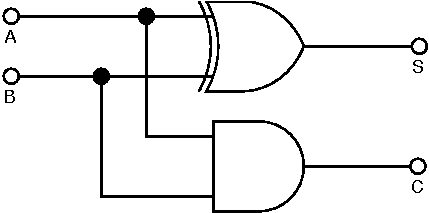
\includegraphics{../diagrams/alu/adder/half_adder.pdf}
        \caption{Logic diagram of the half adder}
    \end{figure}

    \paragraph{Testing}
    \hfill\\\\
    All possible inputs for the half adder are stimulated by the test bench
    and are compared to the expected outputs according to the following
    table:

    \begin{center}
        \begin{tabular}{|c|c||c|c|}
            \hline
            A & B & S & C
            \\\hline\hline
            0 & 0 & 0 & 0
            \\\hline
            1 & 0 & 1 & 0
            \\\hline
            0 & 1 & 1 & 0
            \\\hline
            1 & 1 & 0 & 1
            \\\hline
        \end{tabular}
    \end{center}

    \begin{figure}[H]
        \centering
        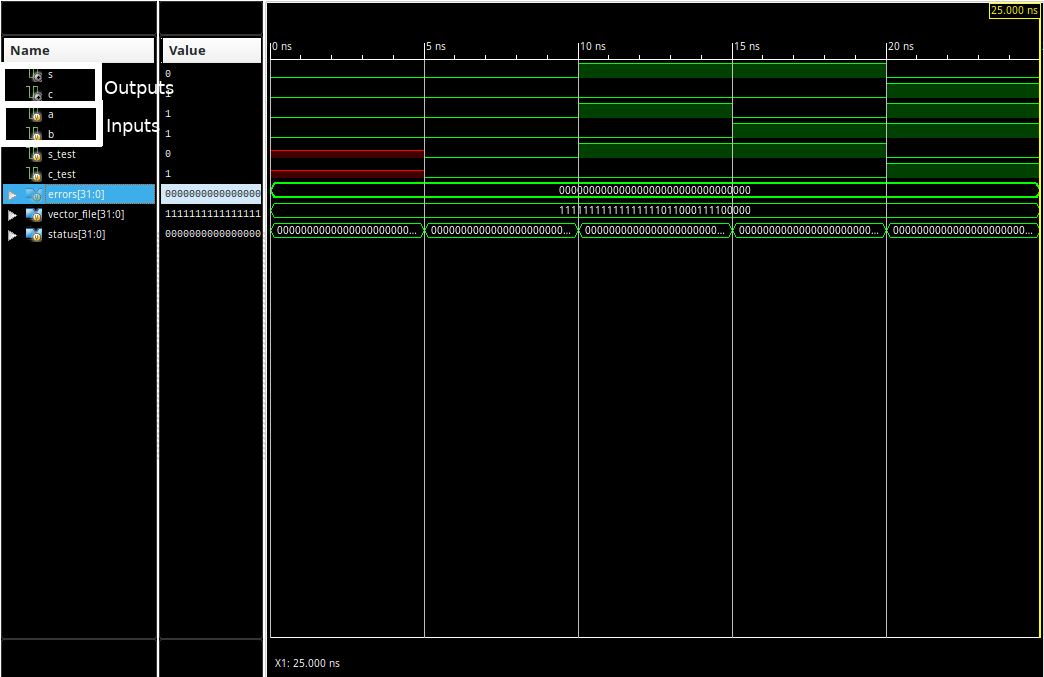
\includegraphics[width=0.9\paperwidth,center]{Screenshots/half_adder.png}
        \caption{Simulation output of half adder}
    \end{figure}



    % Full Adder Module

    \subsubsection{Full Adder}

    \paragraph{Inputs}
    \begin{itemize}
        \item Operand A - 1 bit
        \item Operand B - 1 bit
        \item Carry In - 1 bit
    \end{itemize}

    \paragraph{Outputs}
    \begin{itemize}
        \item Sum - 1 bit
        \item Carry Out - 1 bit
    \end{itemize}

    \paragraph{Functionality}
    \hfill\\\\
    Takes three single bit operands and produces the single bit sum and the
    carry bit.

    \paragraph{Diagrams}
    \hfill\\\\
    \begin{figure}[H]
        \centering
        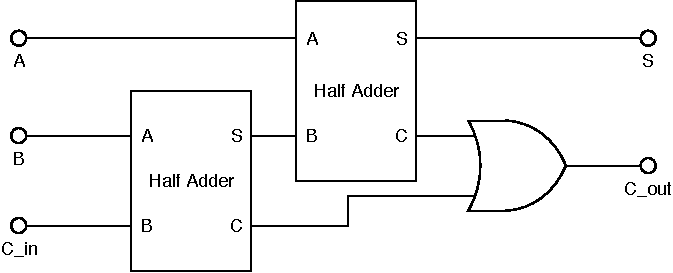
\includegraphics{../diagrams/alu/adder/full_adder.pdf}
        \caption{Logic diagram of the full adder}
    \end{figure}

    \paragraph{Testing}
    \hfill\\\\
    All possible inputs for the full adder are stimulated by the test bench
    and are compared to the expected outputs according to the following
    table:

    \begin{center}
        \begin{tabular}{|c|c|c||c|c|}
            \hline
            A & B & Carry In & S & Carry Out
            \\\hline\hline
            0 & 0 & 0 & 0 & 0
            \\\hline
            1 & 0 & 0 & 1 & 0
            \\\hline
            0 & 1 & 0 & 1 & 0
            \\\hline
            1 & 1 & 0 & 0 & 1
            \\\hline
            0 & 0 & 1 & 1 & 0
            \\\hline
            1 & 0 & 1 & 0 & 1
            \\\hline
            0 & 1 & 1 & 0 & 1
            \\\hline
            1 & 1 & 1 & 1 & 1
            \\\hline
        \end{tabular}
    \end{center}

    \begin{figure}[H]
        \centering
        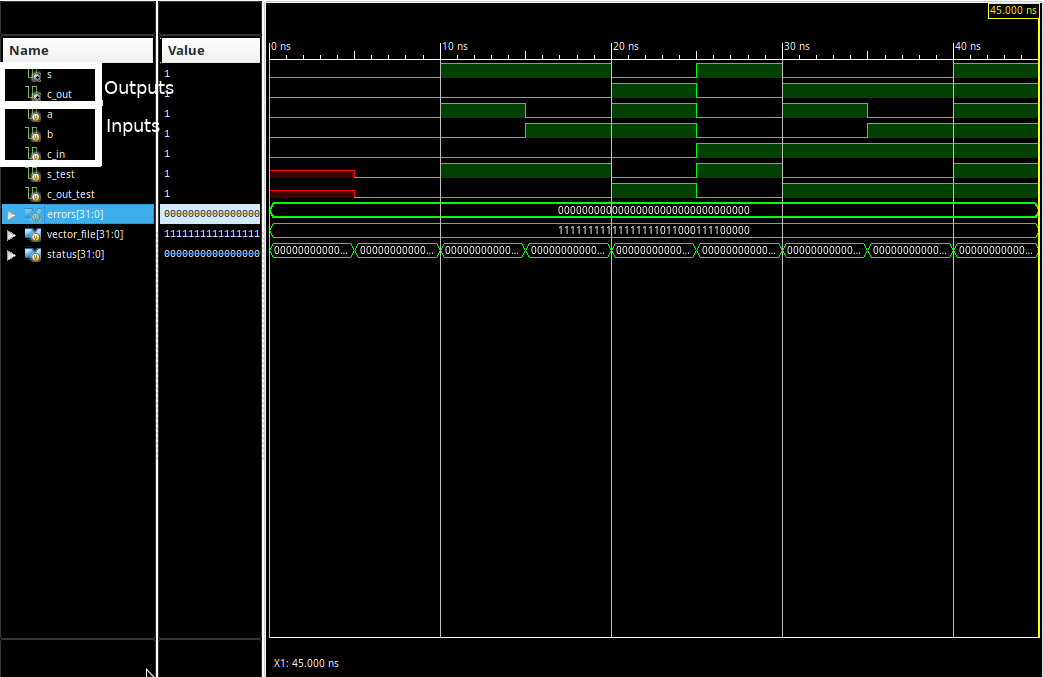
\includegraphics[width=0.9\paperwidth,center]{Screenshots/full_adder.png}
        \caption{Simulation output of full adder}
    \end{figure}



    % 2 Bit Adder Module

    \subsubsection{2 Bit Adder}

    \paragraph{Inputs}
    \begin{itemize}
        \item Operand A - 2 bit
        \item Operand B - 2 bit
        \item Carry In - 1 bit
    \end{itemize}

    \paragraph{Outputs}
    \begin{itemize}
        \item Sum - 2 bit
        \item Carry Out - 1 bit
    \end{itemize}

    \paragraph{Functionality}
    \hfill\\\\
    Takes two 2 bit operands and a third single bit operand and produces the
    2 bit sum and the carry bit.

    \paragraph{Diagrams}
    \hfill\\\\
    \begin{figure}[H]
        \centering
        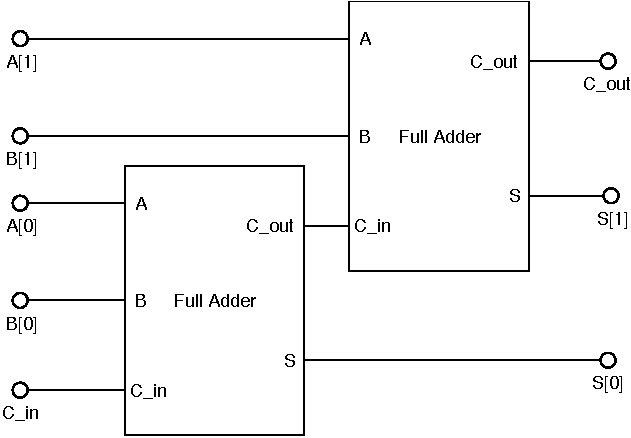
\includegraphics{../diagrams/alu/adder/adder_2.pdf}
        \caption{Logic diagram of the 2 bit adder}
    \end{figure}

    \paragraph{Testing}
    \hfill\\\\
    Due to the larger range of possible inputs, inputs are selected to include
    several base cases, as well as the maximum input value case and minimum
    input value case. The inputs and expected outputs are as follows:

    \begin{center}
        \begin{tabular}{|c|c|c||c|c|}
            \hline
            A & B & Carry In & S & Carry Out
            \\\hline\hline
            3 & 3 & 0 & 2 & 1
            \\\hline\hline
            3 & 1 & 0 & 0 & 1
            \\\hline\hline
            3 & 3 & 1 & 3 & 1
            \\\hline\hline
            0 & 0 & 0 & 0 & 0
            \\\hline
        \end{tabular}
    \end{center}

    \begin{figure}[H]
        \centering
        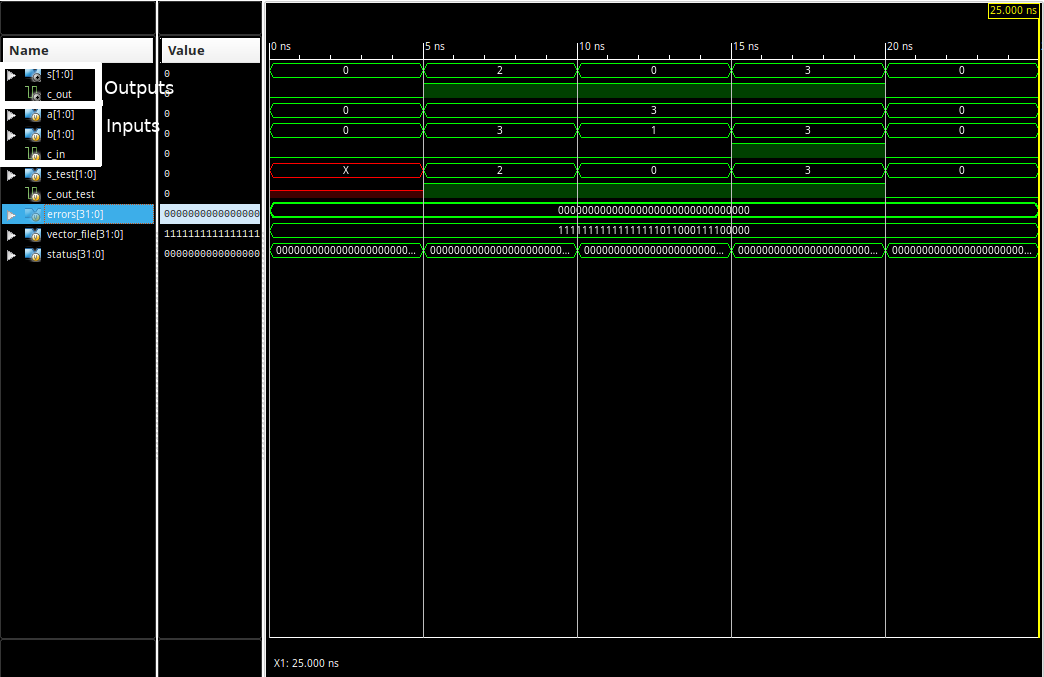
\includegraphics[width=0.9\paperwidth,center]{Screenshots/adder_2.png}
        \caption{Simulation output of 2 bit adder}
    \end{figure}



    % 4 Bit Adder Module

    \subsubsection{4 Bit Adder}

    \paragraph{Inputs}
    \begin{itemize}
        \item Operand A - 4 bit
        \item Operand B - 4 bit
        \item Carry In - 1 bit
    \end{itemize}

    \paragraph{Outputs}
    \begin{itemize}
        \item Sum - 4 bit
        \item Carry Out - 4 bit
    \end{itemize}

    \paragraph{Functionality}
    \hfill\\\\
    Takes two 4 bit operands and a third single bit operand and produces the
    4 bit sum and the carry bit.

    \paragraph{Diagrams}
    \hfill\\\\
    \begin{figure}[H]
        \centering
        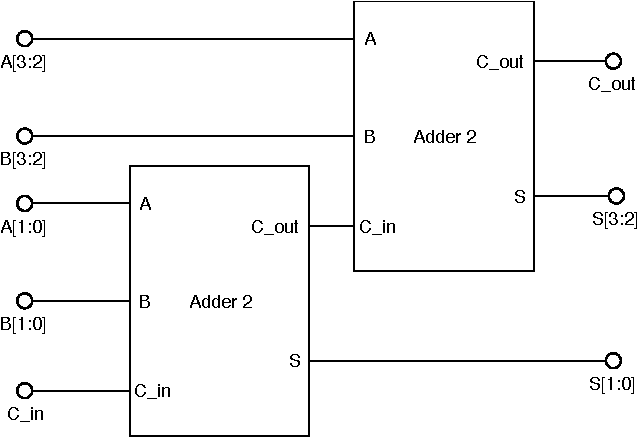
\includegraphics{../diagrams/alu/adder/adder_4.pdf}
        \caption{Logic diagram of the 4 bit adder}
    \end{figure}

    \paragraph{Testing}
    \hfill\\\\
    As this module follows a nearly identical functionality as the 2
    bit adder, and nearly identical Verilog code, testing was ommitted.
    This module's test is included within the 32 bit adder test, as the
    32 bit adder will only function correctly if this module functions
    correctly.




    % 8 Bit Adder Module

    \subsubsection{8 Bit Adder}

    \paragraph{Inputs}
    \begin{itemize}
        \item Operand A - 8 bit
        \item Operand B - 8 bit
        \item Carry In - 1 bit
    \end{itemize}

    \paragraph{Outputs}
    \begin{itemize}
        \item Sum - 8 bit
        \item Carry Out - 8 bit
    \end{itemize}

    \paragraph{Functionality}
    \hfill\\\\
    Takes two 8 bit operands and a third single bit operand and produces the
    8 bit sum and the carry bit.

    \paragraph{Diagrams}
    \hfill\\\\
    \begin{figure}[H]
        \centering
        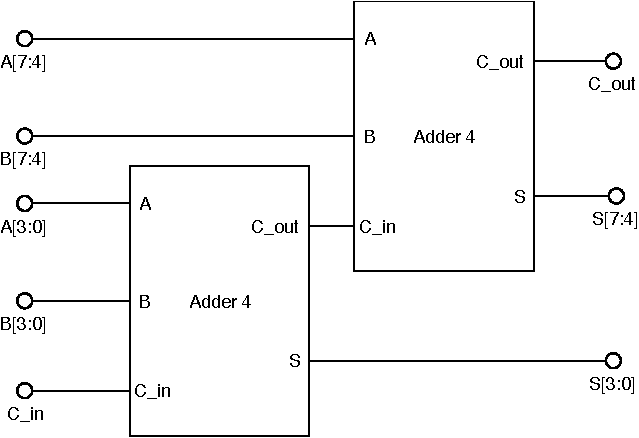
\includegraphics{../diagrams/alu/adder/adder_8.pdf}
        \caption{Logic diagram of the 8 bit adder}
    \end{figure}

    \paragraph{Testing}
    \hfill\\\\
    As this module follows a nearly identical functionality as the 2
    bit adder, and nearly identical Verilog code, testing was ommitted.
    This module's test is included within the 32 bit adder test, as the
    32 bit adder will only function correctly if this module functions
    correctly.




    % 16 Bit Adder Module

    \subsubsection{16 Bit Adder}

    \paragraph{Inputs}
    \begin{itemize}
        \item Operand A - 16 bit
        \item Operand B - 16 bit
        \item Carry In - 1 bit
    \end{itemize}

    \paragraph{Outputs}
    \begin{itemize}
        \item Sum - 16 bit
        \item Carry Out - 16 bit
    \end{itemize}

    \paragraph{Functionality}
    \hfill\\\\
    Takes two 16 bit operands and a third single bit operand and produces the
    16 bit sum and the carry bit.

    \paragraph{Diagrams}
    \hfill\\\\
    \begin{figure}[H]
        \centering
        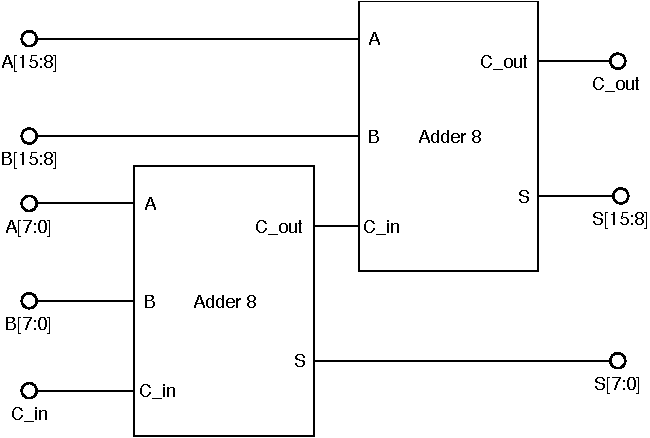
\includegraphics{../diagrams/alu/adder/adder_16.pdf}
        \caption{Logic diagram of the 16 bit adder}
    \end{figure}

    \paragraph{Testing}
    \hfill\\\\
    As this module follows a nearly identical functionality as the 2
    bit adder, and nearly identical Verilog code, testing was ommitted.
    This module's test is included within the 32 bit adder test, as the
    32 bit adder will only function correctly if this module functions
    correctly.



    % 32 Bit Adder Module

    \subsubsection{32 Bit Adder}

    \paragraph{Inputs}
    \begin{itemize}
        \item Operand A - 32 bit
        \item Operand B - 32 bit
        \item Carry In - 1 bit
    \end{itemize}

    \paragraph{Outputs}
    \begin{itemize}
        \item Sum - 32 bit
        \item Carry Out - 32 bit
    \end{itemize}

    \paragraph{Functionality}
    \hfill\\\\
    Takes two 32 bit operands and a third single bit operand and produces the
    32 bit sum and the carry bit.

    \paragraph{Diagrams}
    \hfill\\\\
    \begin{figure}[H]
        \centering
        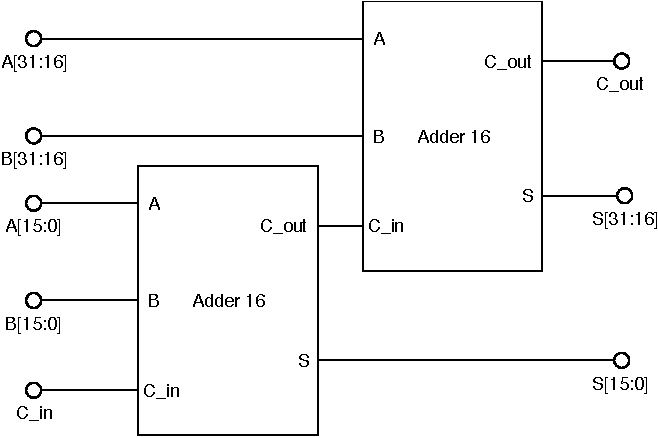
\includegraphics{../diagrams/alu/adder/adder_32.pdf}
        \caption{Logic diagram of the 32 bit adder}
    \end{figure}

    \paragraph{Testing}
    \hfill\\\\
    Due to the larger range of possible inputs, inputs are selected to include
    several base cases, as well as the maximum input value case. The inputs
    and expected outputs are as follows:

    \begin{center}
        \begin{tabular}{|c|c|c||c|c|}
            \hline
            A & B & Carry In & S & Carry Out
            \\\hline\hline
            10 & 10 & 1 & 21 & 0
            \\\hline
            1 & 0 & 1 & 2 & 0
            \\\hline
            4294967295 & 0 & 1 & 0 & 1
            \\\hline
            4294967295 & 4294967295 & 1 & 4294967295 & 1
            \\\hline
        \end{tabular}
    \end{center}

    \begin{figure}[H]
        \centering
        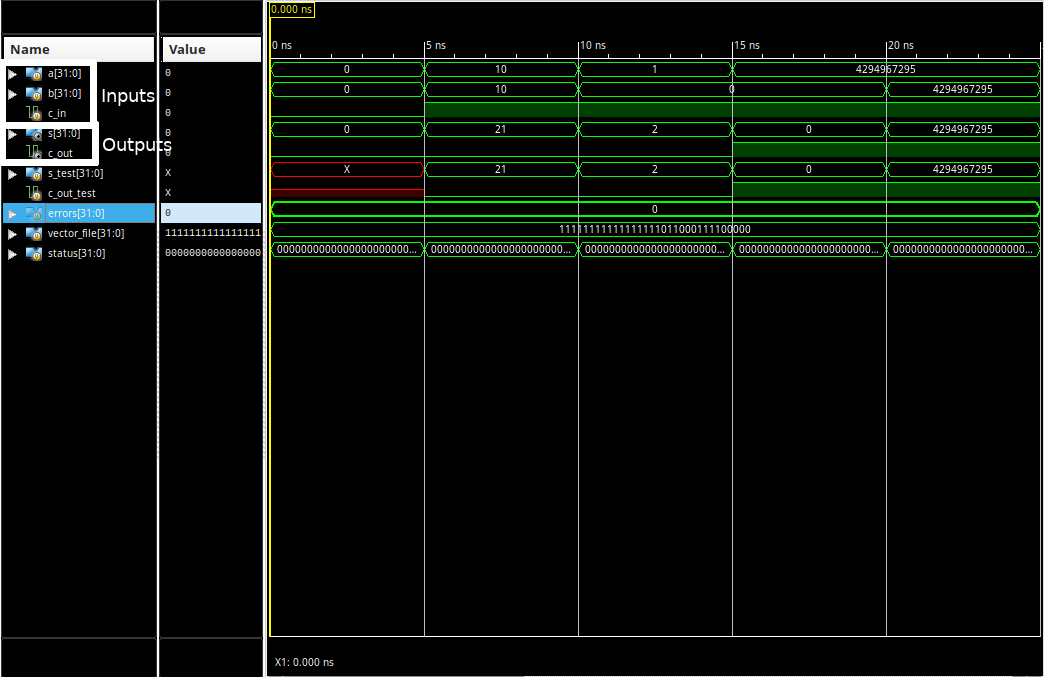
\includegraphics[width=0.9\paperwidth,center]{Screenshots/adder_32.png}
        \caption{Simulation output of 32 bit adder}
    \end{figure}



    \subsection{32 Bit Multiplier}

    \paragraph{Inputs}
    \begin{itemize}
        \item Operand A - 32 bit
        \item Operand B - 32 bit
        \item Clock Signal - 1 bit
        \item Enable Signal - 1 bit
        \item Reset Signal - 1 bit
    \end{itemize}

    \paragraph{Outputs}
    \begin{itemize}
        \item Product - 64 bit
        \item Done Signal - 1 bit
    \end{itemize}

    \paragraph{Functionality}
    \hfill\\
    The multiplier module uses a simple multiplication algorithm, optimized
    to use the minimum number of gates. As a consequence, the multiplier
    module takes multiple clock cycles to complete an operation.

    On the positive edge of the reset signal, the values of operand A
    and operand B are stored by the multiplier and the multiplication is
    reset, but no actual multiplication is performed.

    If the enable signal is high, then on the positive edge of the clock
    signal the module will complete one cycle of the multiplication 
    operation. During this time the product output will change, but it will
    not be the correct value.

    Once the multiplication is complete, the output done signal will be driven
    high and the product will be accurate.

    This module supports signed multiplication.

    \paragraph{Diagrams}
    \hfill\\\\
    \begin{figure}[H]
        \centering
        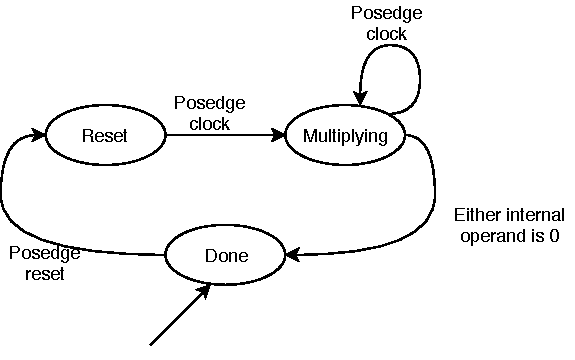
\includegraphics{../diagrams/alu/multiplier/multiplier_32.pdf}
        \caption{State change diagram of the 32 bit multiplier}
    \end{figure}

    \paragraph{Testing}
    \hfill\\\\
    A few base cases are tested with positive and negative number
    multiplication, multiplication by zero, and the largest positive
    inputs and largest negative inputs are tested. Overflow is not tested,
    as with a 64 bit product, overflow is impossible. The inputs and expected
    outputs are as follows:

    \begin{center}
        \begin{tabular}{|c|c||c|}
            \hline
            A & B & Product
            \\\hline\hline
            5 & 10 & 50
            \\\hline
            7 & 5 & 35
            \\\hline
            0 & 0 & 0
            \\\hline
            1 & 0 & 0
            \\\hline
            1 & 1 & 1
            \\\hline
            1 & -1 & -1
            \\\hline
            -1 & -1 & 1
            \\\hline
            2147483647 & 2147483647 & 4611686014132420609
            \\\hline
            -2147483648 & -2147483648 & 4611686018427387904
            \\\hline
        \end{tabular}
    \end{center}


    \begin{figure}[H]
        \centering
        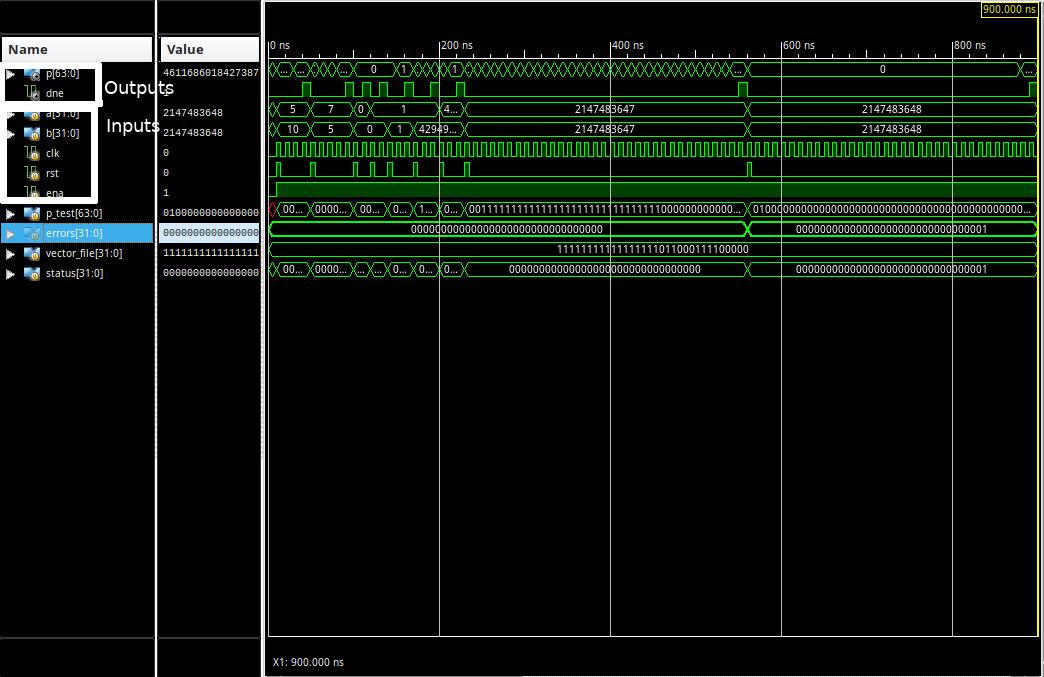
\includegraphics[width=0.9\paperwidth,center]{Screenshots/multiplier_32.png}
        \caption{Simulation output of 32 bit multiplier}
    \end{figure}




    \subsection{32 Bit Divider}

    \paragraph{Inputs}
    \begin{itemize}
        \item Dividend - 32 bit
        \item Divisor - 32 bit
        \item Clock Signal - 1 bit
        \item Enable Signal - 1 bit
        \item Reset Signal - 1 bit
    \end{itemize}

    \paragraph{Outputs}
    \begin{itemize}
        \item Quotient - 32 bit
        \item Remainder - 32 bit
        \item Done Signal - 1 bit
    \end{itemize}

    \paragraph{Functionality}
    \hfill\\
    The multiplier module uses a simple division algorithm, optimized
    to use the minimum number of gates. As a consequence, the divsion
    module takes multiple clock cycles to complete an operation.

    On the positive edge of the reset signal, the values of the dividend
    and divisor are stored by the multiplier and the division is
    reset, but no actual division is performed.

    If the enable signal is high, then on the positive edge of the clock
    signal the module will complete one cycle of the division 
    operation. During this time the quotient output and remainder outputs
    will change, but it will not be the correct value.

    Once the division is complete, the output done signal will be driven
    high and the quotient and remainder will be accurate.

    This module supports signed division.

    \paragraph{Diagrams}
    \hfill\\\\
    \begin{figure}[H]
        \centering
        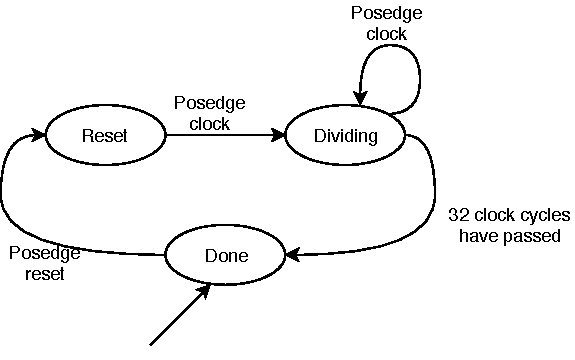
\includegraphics{../diagrams/alu/divider/divider_32.pdf}
        \caption{State change diagram of the 32 bit multiplier}
    \end{figure}

    \paragraph{Testing}
    \hfill\\\\
    A few base cases are tested with positive and negative number
    division inputs and largest negative inputs are tested. Division by 0 is not
    handled. The inputs and expected
    outputs are as follows:

    \begin{center}
        \begin{tabular}{|c|c||c|c|}
            \hline
            A & B & Quotient & Remainder
            \\\hline\hline
            100 & 25 & 4 & 0
            \\\hline
            175 & 100 & 1 & 75
            \\\hline
            10 & 10000 & 0 & 10
            \\\hline
            0 & 1 & 0 & 0
            \\\hline
            1 & 1 & 1 & 0
            \\\hline
            -1 & 1 & -1 & 0
            \\\hline
            -1 & -1 & 1 & 0
            \\\hline
        \end{tabular}
    \end{center}


    \begin{figure}[H]
        \centering
        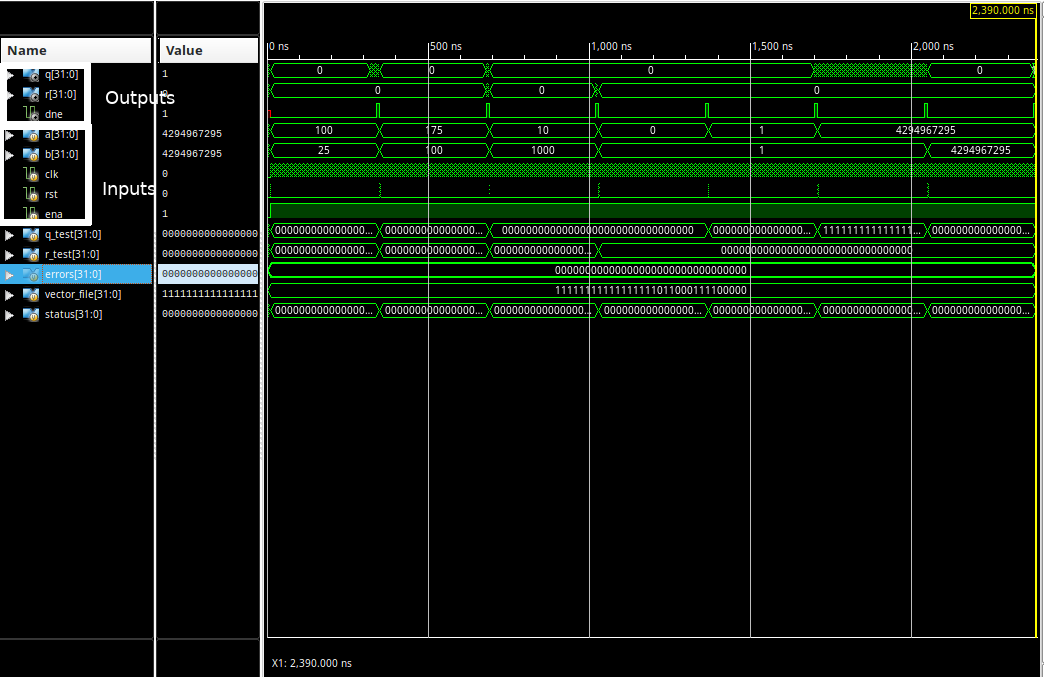
\includegraphics[width=0.9\paperwidth,center]{Screenshots/divider_32.png}
        \caption{Simulation output of 32 bit multiplier}
    \end{figure}



    \subsection{32 Bit ALU}

    \paragraph{Inputs}
    \begin{itemize}
        \item Operand A - 32 bit
        \item Operand B - 32 bit
        \item Operation - 3 bit
        \item Clock Signal - 1 bit
        \item Enable Signal - 1 bit
        \item Reset Signal - 1 bit
    \end{itemize}

    \paragraph{Outputs}
    \begin{itemize}
        \item Result - 32 bit
        \item Extra - 32 bit
        \item Done Signal - 1 bit
    \end{itemize}

    \paragraph{Functionality}
    \hfill\\
    The 32 bit ALU utilizes the 32 bit adder, multiplier, and divider modules
    described above. A multiplexer is used to select the appropriate output
    from the module, depending on the operation code used.

    As this module implements a multiplier and divider that take several
    clock cycles to complete, this ALU requires a reset and clock signal.
    On the positive edge of the reset signal the values of the operands
    are stored and the reset for the arithmetic submodule is triggered.

    Because a multiplexer is used, the operation code must remain constant
    throughout the duration of the operation. Like the multiplier and
    divider, a done signal is driven high on the completion of any operation.

    The lower 32 bits of the operation result are stored in the result output,
    while any additional operation results are stored in the extra output.
    This includes the carry/borrow bit from the addition/subtraction
    operation, the upper 32 bits of the product, or the 32 bits of the
    remainder.

    The subtraction operation is implemented by taking the inverse of the
    second operand and driving the adder's carry in high.

    The different codes for operations are as follows:

    \begin{center}
        \begin{tabular}{|c|c|}
            \hline
            Operation & Code
            \\\hline\hline
            Add & 0
            \\\hline
            Subtract & 1
            \\\hline
            Multiply & 2
            \\\hline
            Divide & 3
            \\\hline
        \end{tabular}
    \end{center}

    \paragraph{Diagrams}
    \hfill\\\\
    \begin{figure}[H]
        \centering
        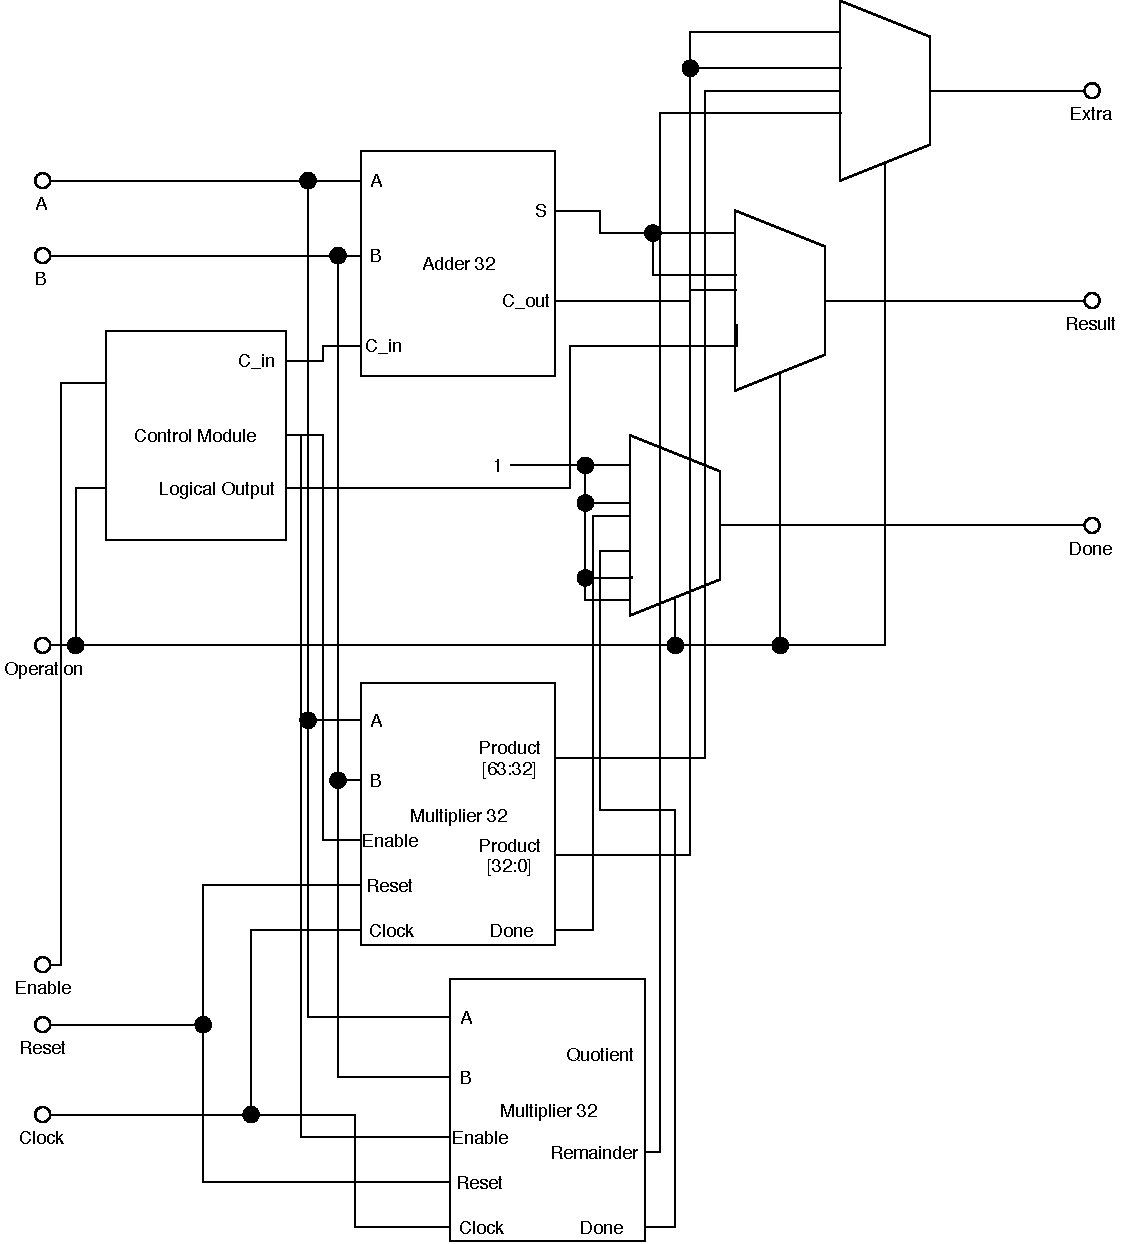
\includegraphics[width=\textwidth]{../diagrams/alu/alu_32.pdf}
        \caption{Logical diagram of the 32 bit ALU}
    \end{figure}

    \paragraph{Testing}
    \hfill\\\\
    As each submodule has been tested individually, only one of each type
    of operation is tested. The inputs and expected outputs are as follows:

    \begin{center}
        \begin{tabular}{|c|c|c||c|c|}
            \hline
            A & B & Operation & Result & Extra
            \\\hline\hline
            1 & 2 & 0 & 3 & 0
            \\\hline
            3 & 4 & 1 & -1 & 0
            \\\hline
            5 & 6 & 2 & 30 & 0
            \\\hline
            7 & 8 & 3 & 0 & 7
            \\\hline
        \end{tabular}
    \end{center}


    \begin{figure}[H]
        \centering
        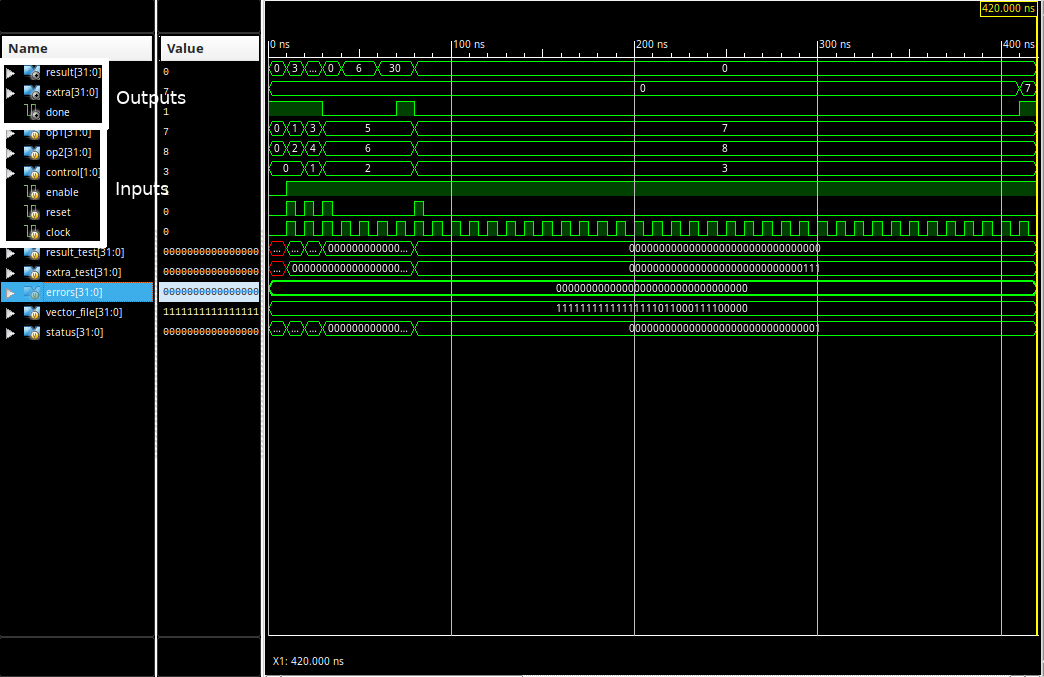
\includegraphics[width=0.9\paperwidth,center]{Screenshots/alu_32.png}
        \caption{Simulation output of 32 bit ALU}
    \end{figure}



    \subsection{Left Shift}

    \paragraph{Inputs}
    \begin{itemize}
        \item Data In - Parameterized Width
    \end{itemize}

    \paragraph{Outputs}
    \begin{itemize}
        \item Data Out - Parameterized Width
    \end{itemize}

    \paragraph{Functionality}
    \hfill\\

    The left shift module is a parameterized module, meaning that it has
    variable width inputs and outputs, as well as variable length shift.
    These parameters are set during instantiation of the module.

    \paragraph{Testing}
    \hfill\\

    A 32 bit left shifter, with a shift amount of 2 is tested. The following
    cases are tested:

    \begin{center}
        \begin{tabular}{|c||c|}
            \hline
            Input & Output
            \\\hline\hline
            00000000000000000000000000000000 & 00000000000000000000000000000000
            \\\hline
            00000000000000000000000000000001 & 00000000000000000000000000000100
            \\\hline
            10000000000000000000000000000000 & 00000000000000000000000000000000
            \\\hline
            11000000000000000000000000000000 & 00000000000000000000000000000000
            \\\hline
        \end{tabular}
    \end{center}


    \begin{figure}[H]
        \centering
        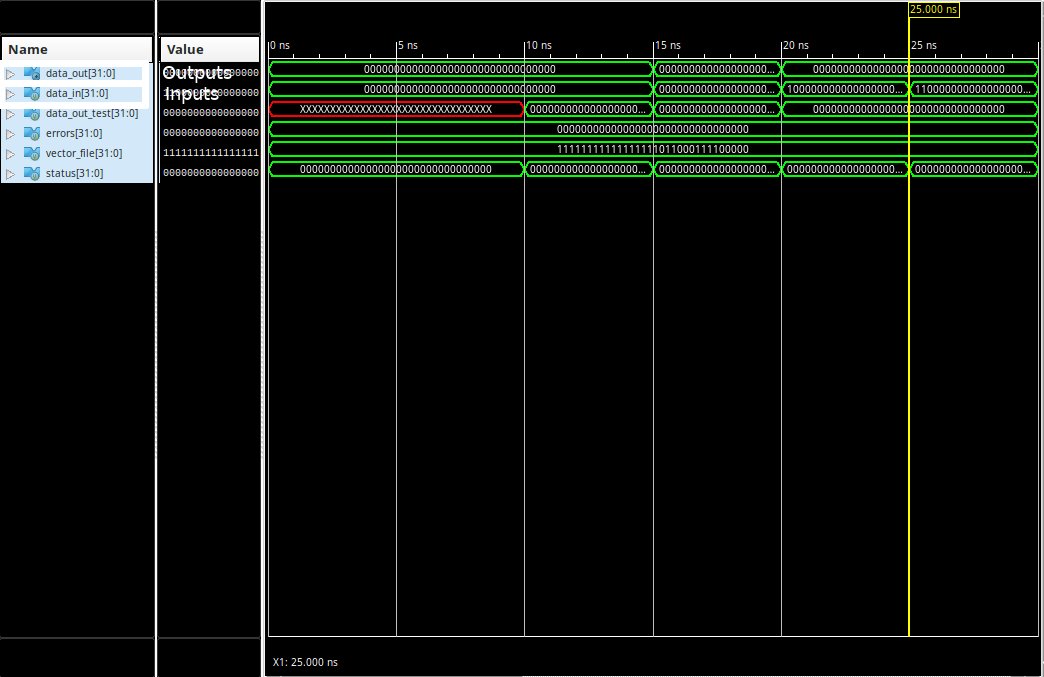
\includegraphics[width=0.9\paperwidth,center]{Screenshots/left_shift.png}
        \caption{Simulation output of 32 bit left shifter}
    \end{figure}



    \subsection{4 Input Multiplexer}

    \paragraph{Inputs}
    \begin{itemize}
        \item Data In 1 - Parameterized Width
        \item Data In 2 - Parameterized Width
        \item Data In 3 - Parameterized Width
        \item Data In 4 - Parameterized Width
        \item Select - 2 bit
    \end{itemize}

    \paragraph{Outputs}
    \begin{itemize}
        \item Data Out - Parameterized Width
    \end{itemize}

    \paragraph{Functionality}
    \hfill\\

    The 4 input multiplexer is a parameterized module, meaning that it has
    variable width inputs and outputs. These parameters are set during
    instantiation of the module.

    This module selects one of four inputs based upon the select signal.

    \paragraph{Testing}
    \hfill\\

    A 32 bit 4 input multiplexer is tested using the following cases:

    \begin{center}
        \begin{tabular}{|c|c|c|c|c||c|}
            \hline
            Data 1 & Data 2 & Data 3 & Data 4 & Select & Output
            \\\hline\hline
            3 & 4 & 5 & 6 & 0 & 3
            \\\hline
            3 & 4 & 5 & 6 & 1 & 4
            \\\hline
            3 & 4 & 5 & 6 & 2 & 5
            \\\hline
            3 & 4 & 5 & 6 & 3 & 6
            \\\hline
            3 & 4 & 5 & 7 & 3 & 7
            \\\hline
        \end{tabular}
    \end{center}


    \begin{figure}[H]
        \centering
        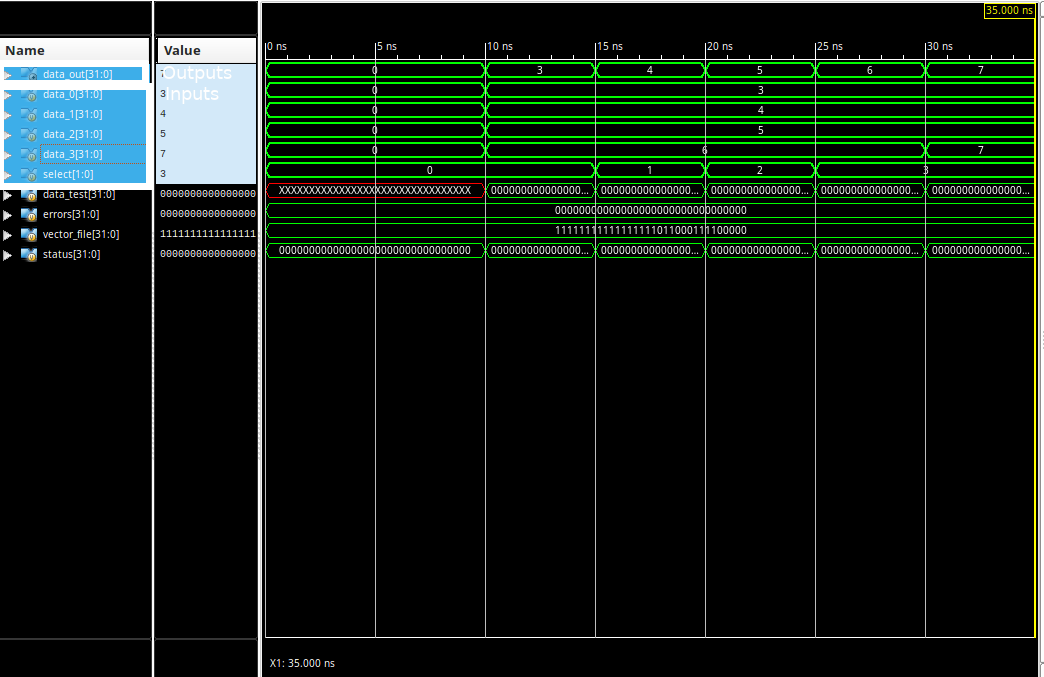
\includegraphics[width=0.9\paperwidth,center]{Screenshots/mux.png}
        \caption{Simulation output of 32 bit 4 input multiplexer}
    \end{figure}



    \subsection{Sign Extender}

    \paragraph{Inputs}
    \begin{itemize}
        \item Data In - Parameterized Width
    \end{itemize}

    \paragraph{Outputs}
    \begin{itemize}
        \item Data Out - Parameterized Width
    \end{itemize}

    \paragraph{Functionality}
    \hfill\\

    The sign extender is a parameterized module, meaning that it has
    variable width inputs and outputs. These parameters are set during
    instantiation of the module.

    This module extends the width of the input data to defined output
    width, maintaining the two's complement sign of the data.

    \paragraph{Testing}
    \hfill\\

    A 16 bit to 32 bit sign extender is tested using the following cases:

    \begin{center}
        \begin{tabular}{|c||c|}
            \hline
            Data In [15:0] & Data Out [31:0]
            \\\hline\hline
            15 & 15
            \\\hline
            -15 & -15
            \\\hline
            255 & 255
            \\\hline
            -255 & -255
            \\\hline
            0 & 0
            \\\hline
        \end{tabular}
    \end{center}


    \begin{figure}[H]
        \centering
        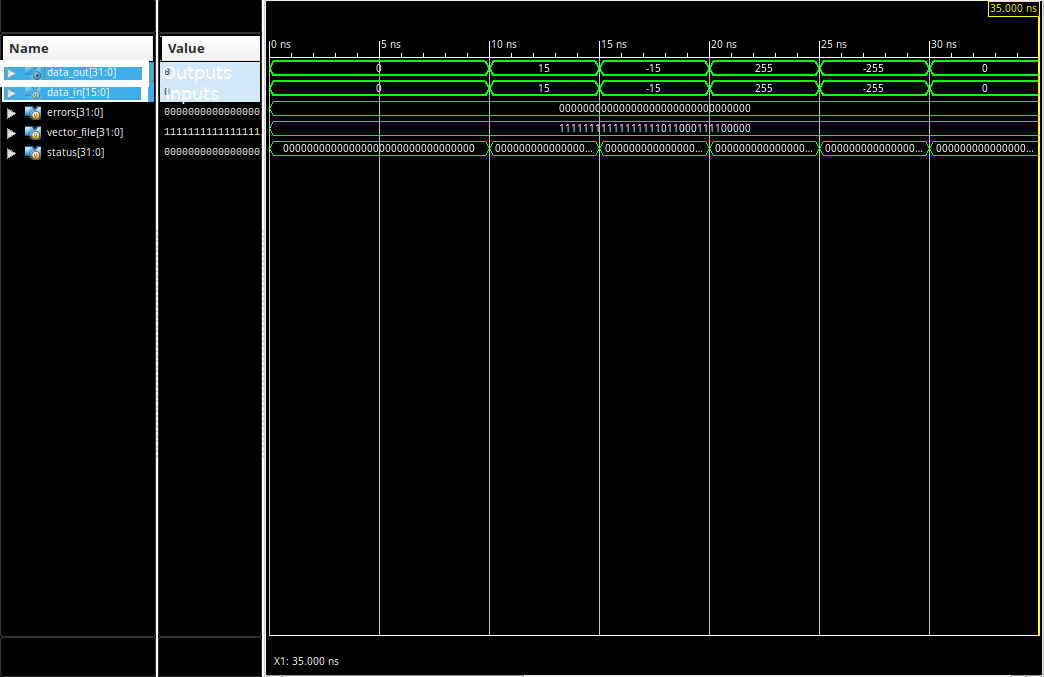
\includegraphics[width=0.9\paperwidth,center]{Screenshots/sign_extend.png}
        \caption{Simulation output of 16 bit to 32 bit sign extender}
    \end{figure}




    \subsection{Register}

    \paragraph{Inputs}
    \begin{itemize}
        \item Read 1 Address - 5 bit
        \item Read 2 Address - 5 bit
        \item Write Enable - 1 bit
        \item Write Address - 5 bit
        \item Data In - 32 bit
    \end{itemize}

    \paragraph{Outputs}
    \begin{itemize}
        \item Data Out 1 - 32 bit
        \item Data Out 2 - 32 bit
    \end{itemize}

    \paragraph{Functionality}
    \hfill\\

    The register module stores 32 different 32 bit values. These values are
    automatically read when either read address is changed. The address
    corresponds to the register index.

    On the positive edge of the write enable signal, the data from data in
    is written to the specified write address.

    \paragraph{Testing}
    \hfill\\

    The register module is tested by first reading the first register to
    ensure that all registers are correctly initialized. Various values
    are written to different registers and then read again to ensure that
    the values were correctly written. The test cases are sequentially as
    follows:

    \begin{center}
        \begin{tabular}{|c|c|c|c|c|}
            \hline
            Read 1 Address & Read 2 Address & Write Enable & Write Address & Data In
            \\\hline\hline
            00 & 00 & 0 & 00 & 00000000
            \\\hline
            00 & 00 & 1 & 01 & ffffffff
            \\\hline
            00 & 01 & 0 & 00 & 00000000
            \\\hline
            01 & 00 & 0 & 02 & dddddddd
            \\\hline
            02 & 01 & 0 & 00 & 00000000
            \\\hline
            01 & 01 & 1 & 02 & bbbbbbbb
            \\\hline
            02 & 01 & 0 & 00 & 00000000
            \\\hline
        \end{tabular}
    \end{center}

    \begin{center}
        \begin{tabular}{|c|c|}
            \hline
            Data 1 Out & Data 2 Out
            \\\hline\hline
            00000000 & 00000000
            \\\hline
            00000000 & 00000000
            \\\hline
            00000000 & ffffffff
            \\\hline
            ffffffff & 00000000
            \\\hline
            00000000 & ffffffff
            \\\hline
            ffffffff & ffffffff
            \\\hline
            bbbbbbbb & ffffffff
            \\\hline
        \end{tabular}
    \end{center}


    \begin{figure}[H]
        \centering
        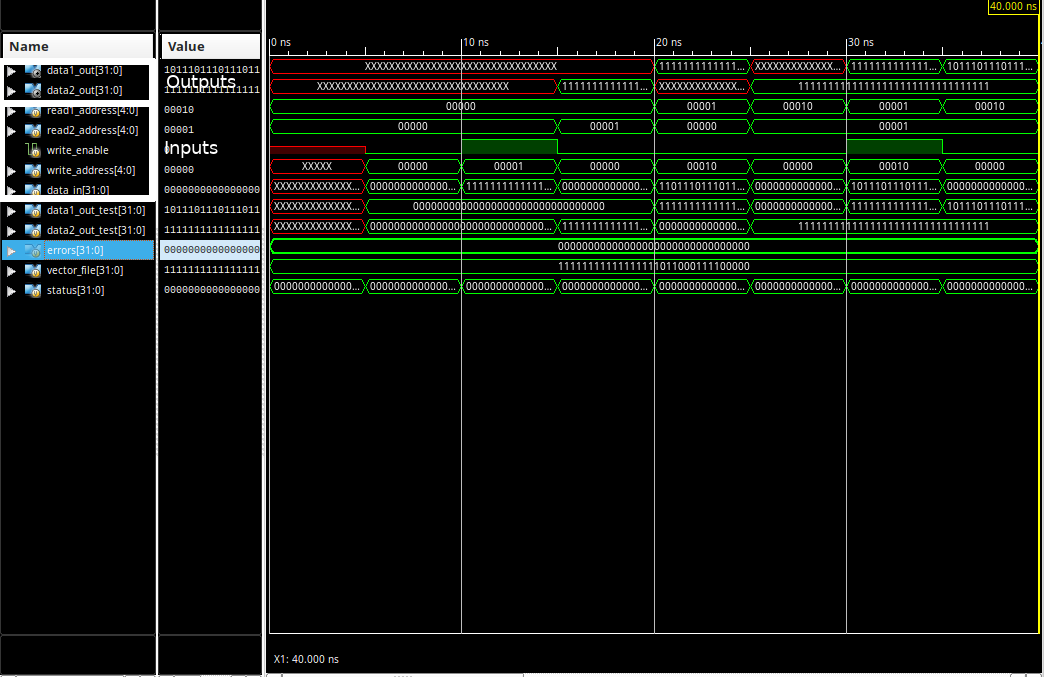
\includegraphics[width=0.9\paperwidth,center]{Screenshots/register.png}
        \caption{Simulation output of the register module}
    \end{figure}


\end{document}